\documentclass[twoside,10pt]{article}
\usepackage{icmc2009,amssymb,amsmath} 
\usepackage[utf8x]{inputenc}
\usepackage[T1]{fontenc}
\usepackage[english]{babel}
\usepackage{color}
%\setcounter{page}{1}

\usepackage{mathptmx} 

\def\papertitle{Goiaba: A music contour processing software}
%\def\papertitle{}	%-- should be empty for the submission anyway!

\def\paperauthorA{} 
\affiliation{}{}


%---- uncomment 1 to 4 lines, for 1 to 4 authors
\def\paperauthorA{Marcos Sampaio}
\def\paperauthorB{Pedro Kröger}
%\def\paperauthorC{Third Author}
%\def\paperauthorD{Fourth Author}

%%---- set correspnding affiliation data for...
%%-- 1 author
%\affiliation{\paperauthorA}
%  {School\\ Department, City, Country \\ {\tt \href{mailto:email@domain.icmc}{email@domain.icmc}}}

%%-- 2 authors with same affiliation
\affiliation{\paperauthorA, \paperauthorB}
 {Genos---Computer Music Research Group\\ School of Music \\ Federal
   University of Bahia, Brazil \\ {\tt
     \href{mailto:mdsmus@gmail.com}{mdsmus@gmail.com} 
     \href{mailto:pedro.kroger@gmail.com}{pedro.kroger@gmail.com}
 }}

%-- 2 authors with different affiliations
%\twoaffiliations{\paperauthorA}{School\\ Department}
%  {\paperauthorB}{Company\\ Address}

%%-- 3 authors with different affiliations
%\threeaffiliations{\paperauthorA}{School A\\ Department X}
%  {\paperauthorB}{Company\\ Address}
%  {\paperauthorC}{School B\\ Department Y}

%%-- 4 authors with different affiliations
%\fouraffiliations{\paperauthorA}{School A\\ Department X}
%  {\paperauthorB}{Company\\ Address}
%  {\paperauthorC}{School B\\ Department Y}
%  {\paperauthorD}{School C\\ Department Z}

%---- the hyperref package must be last to properly work
\usepackage[pdftex,
       pdftitle={\papertitle},
	pdfauthor={\paperauthorA},
	colorlinks=false,bookmarksnumbered,pdfstartview=XYZ]{hyperref}
%\pdfcompresslevel=9
\usepackage[pdftex]{graphicx}	% for compatible graphics with hyperref
\usepackage[figure,table]{hypcap}	% corrects the hyper-anchor of figures/tables
\usepackage{subfig}

../newcommand.tex

\title{\papertitle}

\begin{document}

\maketitle

\begin{abstract}
Contour is the shape or format of objects. Contours can be associated
to musical parameters such as pitch and time, representing one in
function of another. Contours help to give coherence to musical piece
and can be used to analyze and to compose music. Contour theories
provide many operations that demand precise mathematical calculations
and graphical representations easy plotting. In this article we
present the \note{mudar desenvolvimento por estado atual} development
of \goiaba{}, a software that assists musicians in contour tasks, like
calculations and graphical representations plotting.

\end{abstract}

\section{Introduction}
\label{sec:introduction}

Contour is the shape or format of an object. In music one can speak of
a pitch contour, density contour, and so on. Contours can easily be
recognized from graphic representation by professionals and laymen
alike \cite{marvin88:generalized}. For instance, Beethoven's Fifth
Symphony's main motive and the corresponding pitch contour are
represented respectively in figures \ref{fig:5a-sinfonia-motivo} and
\ref{fig:c-3120}.

\begin{figure}[h!]
  \centering
  \subfloat[Main motive]{
    \includegraphics[scale=.9]{5a-sinfonia}
    \label{fig:5a-sinfonia-motivo}
  }

  \subfloat[Contour F(3 1 2 0)]{
    \includegraphics{c-3120}
    \label{fig:c-3120}
  }
  \caption{Fifth Symphony main motive contour}
  \label{fig:5a-sinfonia}
\end{figure}

Technically, a contour is an ordered set of numbered elements
\cite{morris93:directions}. Absolute values of contour elements are
ignored, and only the high-low relationship between them is regarded.
For instance, the music in figures \ref{fig:5a-sinfonia-motivo} and
\ref{fig:ly-3120} have the same pitch contour, graphically represented
in figure \ref{fig:c-3120}, and symbolically by F(3 1 2
0)\footnote{The uppercase letter F names the contour.}. Yet, both
passages sound completely different. In our opinion that is a feature
in using contour theory in composition, to have an underlining process
providing coherence and musical variety at the same time.

The study of contour is important because contours can help to give
coherence to a musical piece, like motives and pitch sets. They are
structural devices that can be combined through operations like
inversion and retrogradation, and can be approached by analytical or
compositional points of view.

\begin{figure}[h!]
  \centering
  \includegraphics{ly-3120-qualquer}
  \caption{A melody with the F(3 1 2 0) contour}
  \label{fig:ly-3120}
\end{figure}

Contour theories
\cite{friedmann85:methodology,friedmann87:response,morris87:composition,morris93:directions,marvin.ea87:relating,marvin88:generalized,polansky.ea92:possible,quinn97:fuzzy,clifford95:contour,beard03:contour}
have been developed to organize the current knowledge about contour in
a systematic way. These theories were developed primarily as analytic
techniques for non-tonal compositions \cite{beard03:contour}, and
provide arrays, matrices and many operations to help the comparison of
contours, like inversion, translation, comparison matrix, and contour
interval array. It's out of the scope of this paper to provide a
comprehensive review about contour theory. The reader can find a good
literature review in \cite{beard03:contour}.

A computer program to process contours can assist composers and
analysts in tasks like the calculation of operations---avoiding human
error and wasting time---, automated graphical plotting, and
conversion from music score to contours and vice-versa. For these
reasons we are developing \goiaba{}\footnote{Goiaba is the Portuguese
  for guava.}, a software to contour processing (described in section
\ref{sec:goiaba}).

In this article we will present \goiaba{}, its data representation,
inputs and outputs, and a case study of a composition, in which
\goiaba{} was used to compose most of a woodwind quintet.

\section{The contour processing program Goiaba}
\label{sec:goiaba}

\goiaba{} is a program written in Common Lisp
\cite{graham94:lisp,team07:sbcl} developed by the authors of this
paper to process and plot contours. It has many contour-related
operations, like inversion, retrogradation, rotation, contour
reduction \cite{adams76:melodic}, contour class, contour adjacency
series, contour adjacency series vector, contour interval, contour
interval array, contour class vector I and II
\cite{friedmann85:methodology}, and comparison matrix
\cite{morris93:directions}. Currently, \goiaba{} accepts and shows
contours in a numeric format, but it can also plot contours in a pdf
file.

\goiaba{} has two representations for contours; simple contours
represents only the values of the contour elements, and contours with
durations are basically ordered collections of cartesian points.  For
instance, the contour in figure \ref{fig:c-3120} would be represented
as a simple contour in \goiaba{} as \code{\#s(3 1 2 0)} and as a
contour with duration as \code{\#d(\#p(0 3) \#p(1 1) \#p(2 2) \#p(3
  0))}. The notations \code{\#s(\ldots)} and \code{\#d(\ldots)}
indicate a simple contour and a contour with duration,
respectively. The notation \code{\#p(x y)} indicates a point with two
values. So, from the example we can see that \goiaba{} really
represents a contour with duration as a collection of points. The
symbols \#s, \#d, and \#p are user-defined lisp reader macros that
expand into code to instantiate objects of types simple-contour,
contour-with-duration, and point, respectively.  For instance,
\code{\#p(0 1)} is expanded to \code{(make-instance 'point :x 0 :y
  1)}, which is the usual way of instantiating objects in common
lisp. Finally, \goiaba{} has a few constructor functions besides the
reader macros to help the creation of contour objects. The functions,
\texttt{make-point-list}, \texttt{make-sim\-ple-contour\-list}, and
\texttt{make-contour-with-du\-ra\-tion-list}, map a list to the
correspondent object.

\goiaba{} uses the Cl-pdf library\footnote{\url{www.cliki.net/CL-PDF}}
to plot contours, allowing easy visualization of contour operations.
For instance, the code in figure \ref{fig:operations-code} generates a
graph with the original contour Z, \code{\#s(0 5 3 4 1 3)}, and its
retrogradation, inversion, and rotation. The result can be seen in
figure \ref{fig:operacoes}.

\begin{figure}
  \centering
\begin{verbatim}
(plot "contour.pdf"
      Z "original Z" :red
      (retrograde Z) "retrograde" :blue
      (inversion Z) "inversion" :orange
      (rotation Z 1) "rotation" :green)
\end{verbatim}
  \caption{Operations code}
  \label{fig:operations-code}
\end{figure}

\begin{figure}
  \centering
  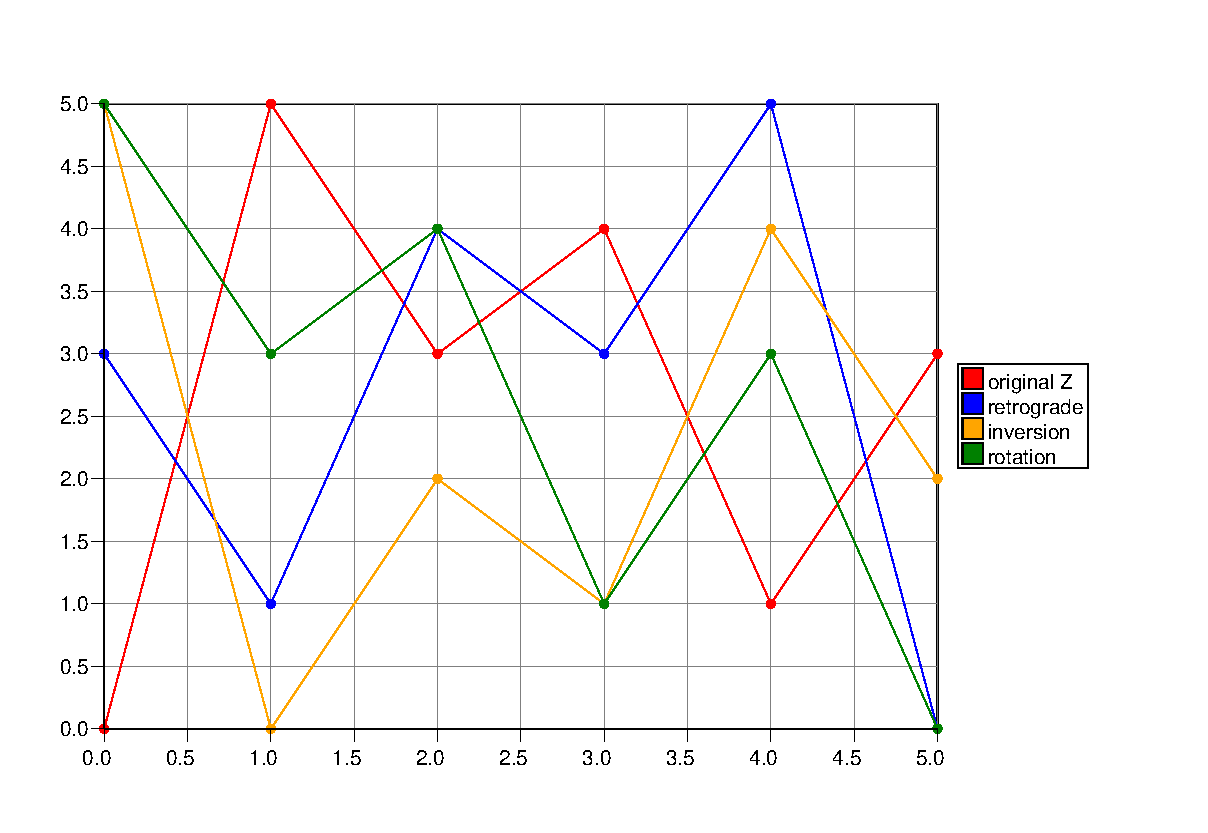
\includegraphics[scale=.44]{contornos}
  \caption{\goiaba{} output: Z(0 5 3 4 1 3) contour operations}
  \label{fig:operacoes}
\end{figure}

\goiaba{} takes advantages of Common Lisp's multimethods capabilities.
In Common Lisp a method is actually a generic function that
specializes on the type of its arguments. For example, we have two
definitions for a generic function called \texttt{rotate}, one
specializes on the contour-with-duration object while the other on the
simple-contour object. The advantage of this approach is that we can
add more types of contour if necessary and write the appropriate
generic functions that will specialize on those types, without
disrupting the existing code.

\begin{figure*}
\begin{verbatim}
(defmethod rotate ((object contour-with-duration) &optional (factor 1))
  (if (> fator (length (points object)))
      (let ((x (mapcar #'point-x (points object)))
            (y (mapcar #'point-y (points object))))
        (make-contour-with-duration (mapcar #'make-point x
           (append (subseq y factor) (subseq y 0 factor)))))))

(defmethod rotate ((object simple-contour) &optional (factor 1))
  (make-simple-contour (append (subseq (points object) factor)
                               (subseq (points object) 0 factor))))
\end{verbatim}
  \caption{Multi-methods}
  \label{fig:code-methods}
\end{figure*}

\section{The application of Contour in composition}
\label{sec:cont-appl-comp}

Systematic studies about the usage of contour operations and
combinations in musical composition are scarce, despite the possible
coherence that contours can provide. For this reason we are
researching the usage of contour in composition and its advantages.
The first author of this paper, during his master's\footnote{The
  reference was removed for anonymity and will be added in the final
  version}
% \cite{sampaio08:em}
, composed a woodwind quintet, 
% \textit{Em Torno da Romã}\footnote{Around the Pomegranate}
based on contour theories operations.

% \textit{Em torno da Romã}
This piece
was composed entirely using \goiaba{} to simplify the calculation of
contour operations and plotting. The piece is based on the contour P(5
3 4 1 2 0) and on combinations of contour operations associated to
parameters such as pitch, tempo, density and texture. In figure
\ref{fig:c-534120} we can see the original contour P and its subsets
and operations; retrogradation, inversion, rotation, and
interpolation.

\begin{figure}
  \centering
  \includegraphics{c-534120}
  \caption{P(5 3 4 1 2 0) contour}
  \label{fig:c-534120}
\end{figure}

\goiaba{} was essential to compose a \eng{fugato} session in the
quintet because each part of the subject and countersubject were based
on different combinations of operations of rotation and
retrogradation. The subject is formed by the concatenation of P and
its rotation by a factor of 3, as seen in figure
\ref{fig:sujeito-fugato}. Figure \ref{fig:output-sujeito-fugato} shows
\goiaba{}'s graphical output for both contours. The countersubject is
formed by a sequence of three rotations (by the factor of 5, 4, and 3)
of the retrograde of P (fig. \ref{fig:contra-sujeito-fugato}). We can
see the graphical output of these contours in figure
\ref{fig:output-contra-sujeito-fugato}.

\begin{figure*}
  \centering
  \subfloat[Subject]{
    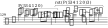
\includegraphics[scale=2.8]{sujeito-fugato}
    \label{fig:sujeito-fugato}
  }

  \subfloat[Counter-subject]{
    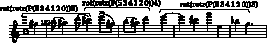
\includegraphics[scale=2.8]{contra-sujeito-fugato}
    \label{fig:contra-sujeito-fugato}
  }
  \caption{Structural elements of \eng{fugato}}
  \label{fig:elementos-fugato}
\end{figure*}

\begin{figure*}
  \centering
  \subfloat[Subject]{
    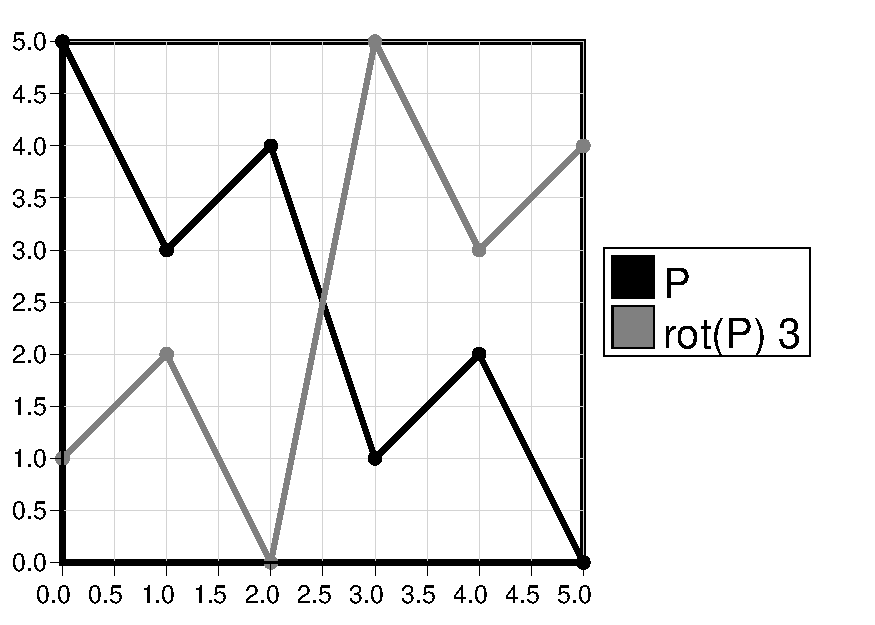
\includegraphics[scale=.44]{output-subject}
    \label{fig:output-sujeito-fugato}
  }
  \subfloat[Counter-subject]{
    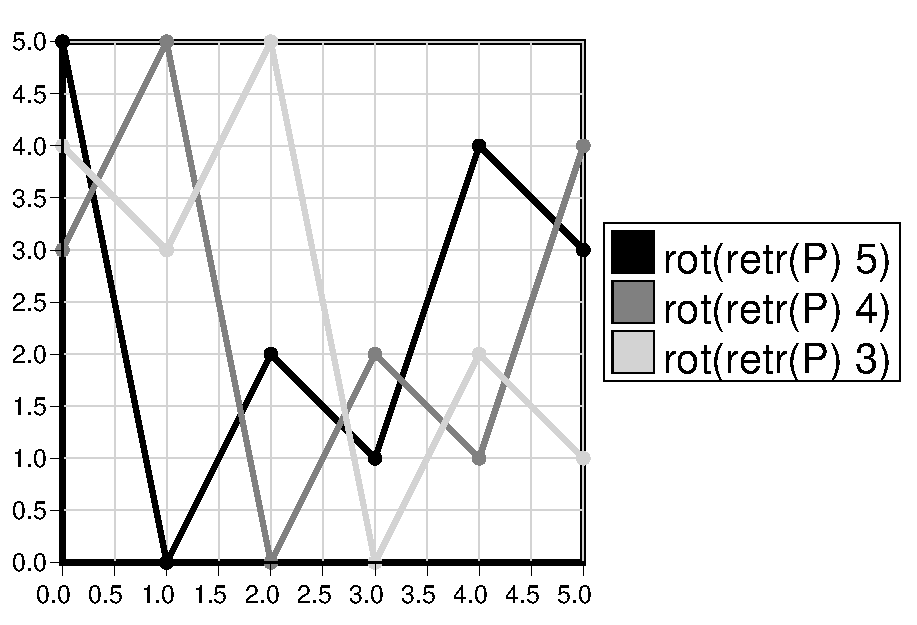
\includegraphics[scale=.44]{output-countersubject}
    \label{fig:output-contra-sujeito-fugato}
  }
  \caption{Software output for \eng{fugato} contour operations}
  \label{fig:output-fugato}
\end{figure*}

\section{Conclusion and future work}
\label{sec:conclusion-future-work}

Contours help to give coherence to a musical piece, are easily
recognized graphically by musicians and laymen, and can be used to
analyze and compose music. Contour theories provide many operations
that demand precise mathematical calculations and graphical
representation, for this reason we are developing \goiaba{}, a contour
processing software that helps the calculation and plotting of contour
operations. \goiaba{} has been proven to be useful in composing music
that uses contour theory extensively. Currently \goiaba{} accepts only
input in a symbolic format, but we have plans to add support for
Lilypond, MIDI, ABC, and MusicXML formats as well. The next step in
our research is to improve \goiaba{} user interaction, releasing a
more friendly interface, possibly with a GUI.

%%% Local Variables: 
%%% mode: latex
%%% TeX-master: "goiaba-contour-processor"
%%% End: 

\bibliographystyle{IEEEtranS}
\bibliography{melodic-contour,music-perception,composition,music-harmony-and-theory,programs,music-analysis,audio,genos,computer-science}


\end{document}
